
                \begin{figure}
                    \centering
                    \begin{tikzpicture}
                        \pgfplotsset{%
                            width=1\textwidth,
                            height=0.4\textheight
                        }
                        \begin{axis}[
                            xlabel={Runs since restart},
                            ylabel={Average dynamic energy (watt)},
                            ymin=0,ymax=70,
                        ]
                        
                            \addplot [mark=none, densely dashed, red]  coordinates {
                            (1, 29.31988512605307)(2, 28.472409388936953)(3, 28.647417166957183)(4, 28.536463089627745)(5, 28.589476892982386)
                            };
                            \addlegendentry{WRK - IPG}
                            
                            \addplot [mark=none, densely dashed, blue]  coordinates {
                            (1, 30.841462981069082)(2, 28.745834086118098)(3, 28.350271131322664)(4, 28.75859151425193)(5, 28.286696336648827)
                            };
                            \addlegendentry{WRK - LHM}
                            
                            \addplot [mark=none, densely dashed, cyan]  coordinates {
                            (1, 16.671237185180534)(2, 25.804294689797715)(3, 19.46855807922392)(4, 17.68514444673619)(5, 26.65591249329199)
                            };
                            \addlegendentry{WRK - CLAMP (win)}
                            
                            \addplot [mark=none, densely dashed, orange]  coordinates {
                            (1, 37.97879118403863)(2, 37.5032167860626)(3, 38.18425151013054)(4, 37.685842260139125)(5, 38.09397223868828)(6, 38.28933773112049)(7, 37.67068201110917)(8, 37.7072866261335)(9, 38.03320267586893)(10, 38.4158037843246)(11, 37.87632818388321)(12, 38.32719094475622)(13, 37.84103785988799)(14, 38.1506380723186)(15, 37.8879637083325)(16, 37.70693799518527)(17, 37.492974903327905)(18, 38.05709100950759)(19, 37.66357745765244)(20, 37.85569500585459)(21, 37.50223886591497)(22, 37.93201947665016)(23, 37.704405770907485)(24, 38.091830122316104)(25, 37.83152602893529)(26, 38.10466625002234)(27, 38.033042041461435)(28, 38.087881838994264)(29, 38.282463543296764)
                            };
                            \addlegendentry{WRK - RAPL}
                            
                            \addplot [mark=none, densely dashed, black]  coordinates {
                            (1, 37.45079912813355)(2, 24.05686086778472)(3, 34.508541683655295)(4, 35.11140415051214)(5, 42.01724956260924)(6, 35.24406304943983)(7, 33.44633576070089)(8, 42.10472043984751)(9, 35.44833114911991)(10, 34.61595768860607)(11, 36.07877637050831)(12, 36.19215753706359)(13, 34.874949356442215)(14, 34.78573013820744)(15, 35.91710659623408)(16, 33.86328590029812)(17, 35.111787638866275)(18, 35.19794396664672)(19, 36.001538903379924)(20, 35.12309028805974)(21, 34.87217711601059)(22, 34.491596317958454)(23, 35.45041388593913)(24, 40.17980818919227)(25, 24.785540795263444)(26, 34.21776954102296)(27, 35.21887895760736)(28, 35.301972221138485)(29, 35.21506895885834)
                            };
                            \addlegendentry{WRK - CLAMP (lin)}
                            
                        \end{axis}
                    \end{tikzpicture} 
                \caption{A graph illustrating the energy consumption of Cores for test case Fasta with regards to how long ago the DUT was restarted, experiment \#2, (with outliers)} \label{fig:Fasta_Cores_iteration_exp2}
                \end{figure}
                